\documentclass{article}

% Packages
\usepackage{amsmath}    
\usepackage{graphicx}   
\usepackage{float}      
\usepackage{booktabs}   
\usepackage{neurips_2024}
\usepackage[utf8]{inputenc}
\usepackage[T1]{fontenc}
\usepackage{hyperref}
\usepackage{url}
\usepackage{amsfonts}
\usepackage{nicefrac}
\usepackage{microtype}
\usepackage{xcolor}

\begin{document}

\title{Support Vector Machines for Credit Default Prediction}


\maketitle

\begin{abstract}
This class project presents an analysis of support vector machines (SVMs) applied to the UCI Default of Credit Card Clients dataset. 
The project explores the impacts of different kernel functions and optimization techniques on classification performance. 
SVMs with linear, radial basis function (RBF), polynomial, and sigmoid kernels are evaluated. 
A grid search approach is used for hyperparameter optimization, and the decision boundary is visualized using Principal Component Analysis (PCA). 
The results are evaluated using accuracy, precision, recall, F1-score, and runtime, demonstrating the utility of SVMs for binary classification tasks on tabular data.
\end{abstract}

\section{Introduction}
Support vector machines are a powerful supervised machine learning approach that have demonstrated robust performance in a wide range of classification tasks. 
This project investigates the application of SVMs to the UCI Default of Credit Card Clients dataset, with a specific focus on assessing the impact of kernel functions 
and optimization techniques on model performance. The study also examines how hyperparameter tuning can enhance SVM efficiency and accuracy, while PCA is employed to 
visualize the decision boundary for improved interpretability. The primary objective of this study is to assess the efficacy of SVMs for predicting credit card default 
and to analyze the computational trade offs associated with various kernel functions and optimization strategies.


\section{Dataset}

The UCI Default of Credit Card Clients dataset is a multivariate dataset containing data from 30,000 credit card holders in Taiwan. 
The dataset is primarily designed for binary classification tasks, specifically predicting whether a client would default on their next month's payment. 
It includes 23 features, which consist of demographic variables such as age, sex, education, and marital status, along with financial metrics like credit limits, 
historical bill statements, and repayment amounts. The target variable is binary, indicating whether a client defaulted (1) or did not default (0) on their credit card payment. 

The dataset includes a mix of categorical and numerical variables. Key variables include repayment statuses (\texttt{PAY\_0} through \texttt{PAY\_6}), 
historical bill amounts (\texttt{BILL\_AMT1} through \texttt{BILL\_AMT6}), and historical repayment amounts (\texttt{PAY\_AMT1} through \texttt{PAY\_AMT6}). 
Additionally, demographic variables such as \texttt{SEX}, \texttt{EDUCATION}, and \texttt{MARRIAGE} provide insights into customer profiles. Table~\ref{variables_table} 
summarizes the features included in the dataset.

\begin{table}[H]
\centering
\caption{Summary of Key Features in the Dataset}
\label{variables_table}
\begin{tabular}{@{}lcll@{}}
\toprule
\textbf{Variable Name} & \textbf{Type} & \textbf{Description}                  & \textbf{Units}       \\ \midrule
SEX                    & Categorical   & Gender                                & 1 = Male, 2 = Female \\
EDUCATION              & Categorical   & Education level                       & 1 = Graduate, etc.   \\
MARRIAGE               & Categorical   & Marital status                        & 1 = Married, etc.    \\
BILL\_AMT1-6           & Numerical     & Monthly bill amounts (6 months)       & NT Dollars           \\
PAY\_AMT1-6            & Numerical     & Historical repayment amounts (6 months) & NT Dollars         \\
PAY\_0-6               & Categorical   & Repayment status (-2: advance payment) & Discrete values      \\
DEFAULT (Target)       & Binary        & Default status for the next month     & 0 = No, 1 = Yes      \\ \bottomrule
\end{tabular}
\end{table}

To prepare the dataset for modeling, extensive preprocessing was conducted. Several variables, such as \texttt{SEX}, \texttt{EDUCATION}, \texttt{MARRIAGE}, 
and repayment statuses (\texttt{PAY\_0} through \texttt{PAY\_6}), were categorical in nature. Since support vector machines require numerical input, 
these categorical variables were transformed into one hot encoded binary variables. This encoding ensured that each category was treated as an independent feature, avoiding implicit ordinal assumptions. 
Furthermore, the dataset exhibited significant class imbalance, with the majority of clients not defaulting on their payments. To address this imbalance, the majority class (non-default clients) 
was downsampled to create a balanced dataset, ensuring that the model learned patterns equally well from both defaulting and non-defaulting clients.

Another essential preprocessing step involved standardizing numerical features, such as bill amounts and repayment amounts. These features had varying scales, with some variables measured in monetary units and others as categorical values. 
Without standardization, features with larger magnitudes could disproportionately influence the model. Therefore, all continuous features were scaled to have a mean of zero and a standard deviation of one, ensuring fair contribution from each variable.

The preprocessing steps of one hot encoding, downsampling, and standardization were necessary to ensure that the dataset was compatible with support vector machines and capable of producing meaningful predictions. 
These transformations addressed the challenges posed by mixed feature types, class imbalance, and variable scaling, ultimately improving the efficiency and accuracy of the machine learning models applied in this study.


\section{Methodology}
After preprocessing the dataset to address class imbalance and ensure numerical compatibility, the project proceeded with training a preliminary Support Vector Machine (SVM) using the radial basis function (RBF) kernel. 
The choice of the RBF kernel for initial experimentation was motivated by its capability to map input features into higher-dimensional spaces, enabling it to capture complex, nonlinear decision boundaries. 
The initial model utilized default hyperparameters, with the regularization parameter \(C = 1\) and kernel coefficient \(\gamma = \frac{1}{\text{number of features}}\), to establish a baseline performance. 
Model evaluation involved generating confusion matrices, as shown in Figure~\ref{fig:confusion-pre-grid}, and calculating accuracy scores.

The SVM optimization process centered around hyperparameter tuning using grid search cross-validation. The grid search method systematically evaluates combinations of \(C\) and \(\gamma\) values to identify the optimal 
hyperparameters that maximize classification performance. The regularization parameter \(C\) controls the trade off between achieving a low training error and maintaining a large margin. The SVM optimization problem is expressed as:

\[
\min_{\mathbf{w}, b, \xi} \frac{1}{2} \|\mathbf{w}\|^2 + C \sum_{i=1}^n \xi_i,
\]

subject to:

\[
y_i (\mathbf{w}^\top \phi(\mathbf{x}_i) + b) \geq 1 - \xi_i, \quad \xi_i \geq 0, \quad i = 1, \dots, n,
\]

where \(\mathbf{w}\) is the weight vector, \(b\) is the bias, \(\xi_i\) are slack variables allowing soft margin violations, and \(\phi(\mathbf{x}_i)\) represents the transformation of input features into a higher-dimensional space. 
The kernel coefficient \(\gamma\) determines the influence of individual training points, effectively controlling the curvature of the decision boundary in the feature space. The post-optimization confusion matrix, 
which demonstrates improved performance, is shown in Figure~\ref{fig:confusion-post-grid}.

To provide a comprehensive analysis, four kernel functions—linear, polynomial, RBF, and sigmoid—were evaluated. Each kernel was optimized using grid search to determine its best performing hyperparameters. 
The linear kernel assumes a straight-line decision boundary and is suitable for datasets that are linearly separable. 

Performance metrics, including accuracy, precision, recall, F1-score, and runtime, were recorded for each kernel to evaluate their suitability for the credit card default prediction task. The accuracy of the SVM models was calculated as:

\[
\text{Accuracy} = \frac{\text{TP} + \text{TN}}{\text{TP} + \text{TN} + \text{FP} + \text{FN}},
\]

where \(\text{TP}\), \(\text{TN}\), \(\text{FP}\), and \(\text{FN}\) represent true positives, true negatives, false positives, and false negatives, respectively. Precision, recall, 
and F1-score were also computed to provide a more detailed assessment of the models' performance in handling class imbalance.

To facilitate visualization and interpretability, Principal Component Analysis (PCA) was employed to reduce the feature space to two dimensions. PCA identifies orthogonal directions, or principal components, 
that capture the maximum variance in the dataset. The decision boundary for each kernel, projected onto the first two principal components, is illustrated in Figure~\ref{fig:decision-surface}. 
The PCA transformed decision boundary provides a visual representation of the separability between defaulting and non-defaulting clients.


\section{Results}
The comparative analysis of kernel functions yielded results, summarized in Table~\ref{kernel-results}. The RBF kernel outperformed other kernels, achieving the highest accuracy (68.75\%) and F1-score (0.65). 
The scree plot in Figure~\ref{fig:scree-plot} highlights the explained variance by the principal components, providing insights into the dimensionality reduction process.

\begin{figure}[H]
    \centering
    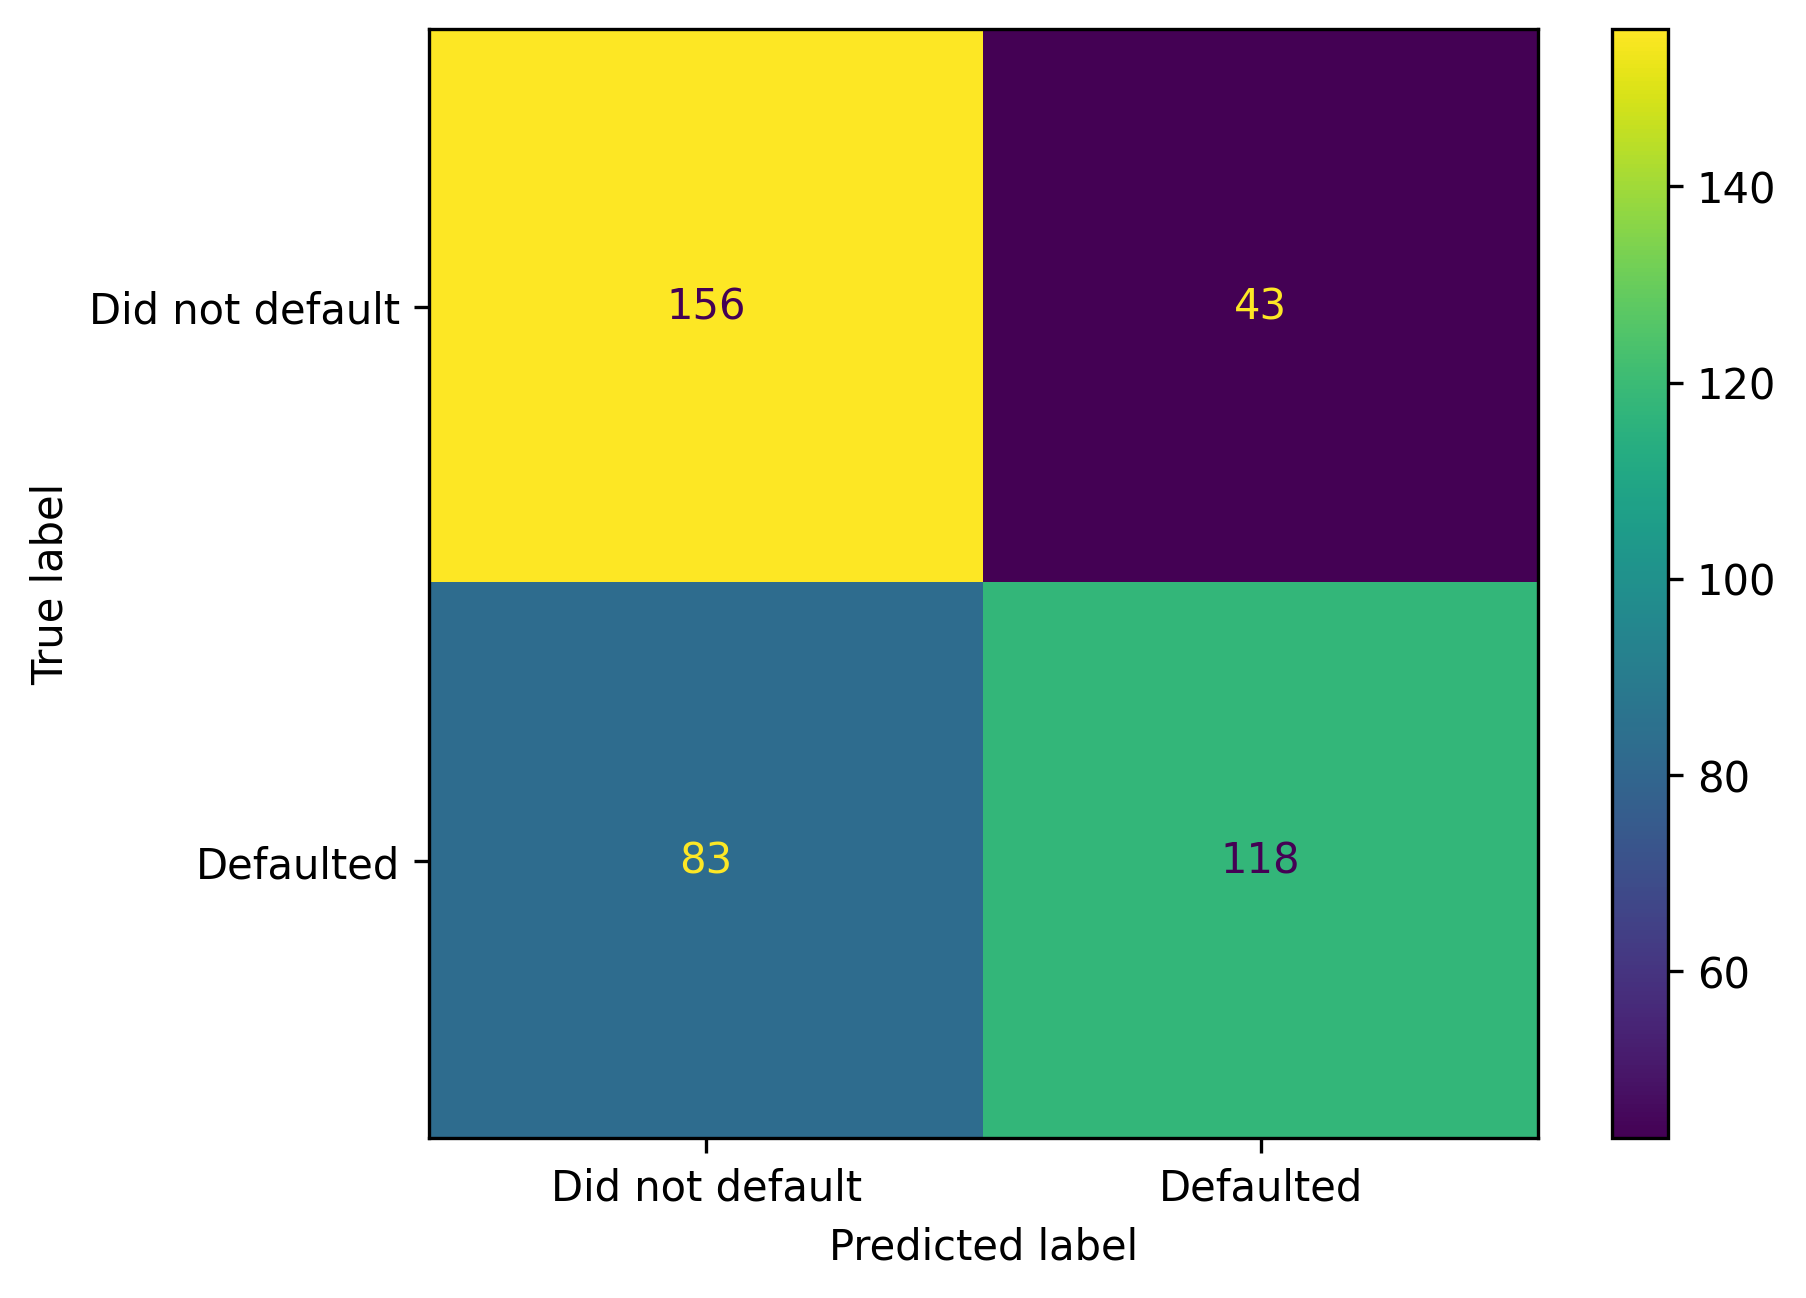
\includegraphics[width=0.7\textwidth]{../figures/confusion_matrix_pre_gridSearch.png}
    \caption{Confusion Matrix Before Grid Search.}
    \label{fig:confusion-pre-grid}
\end{figure}

\begin{figure}[H]
    \centering
    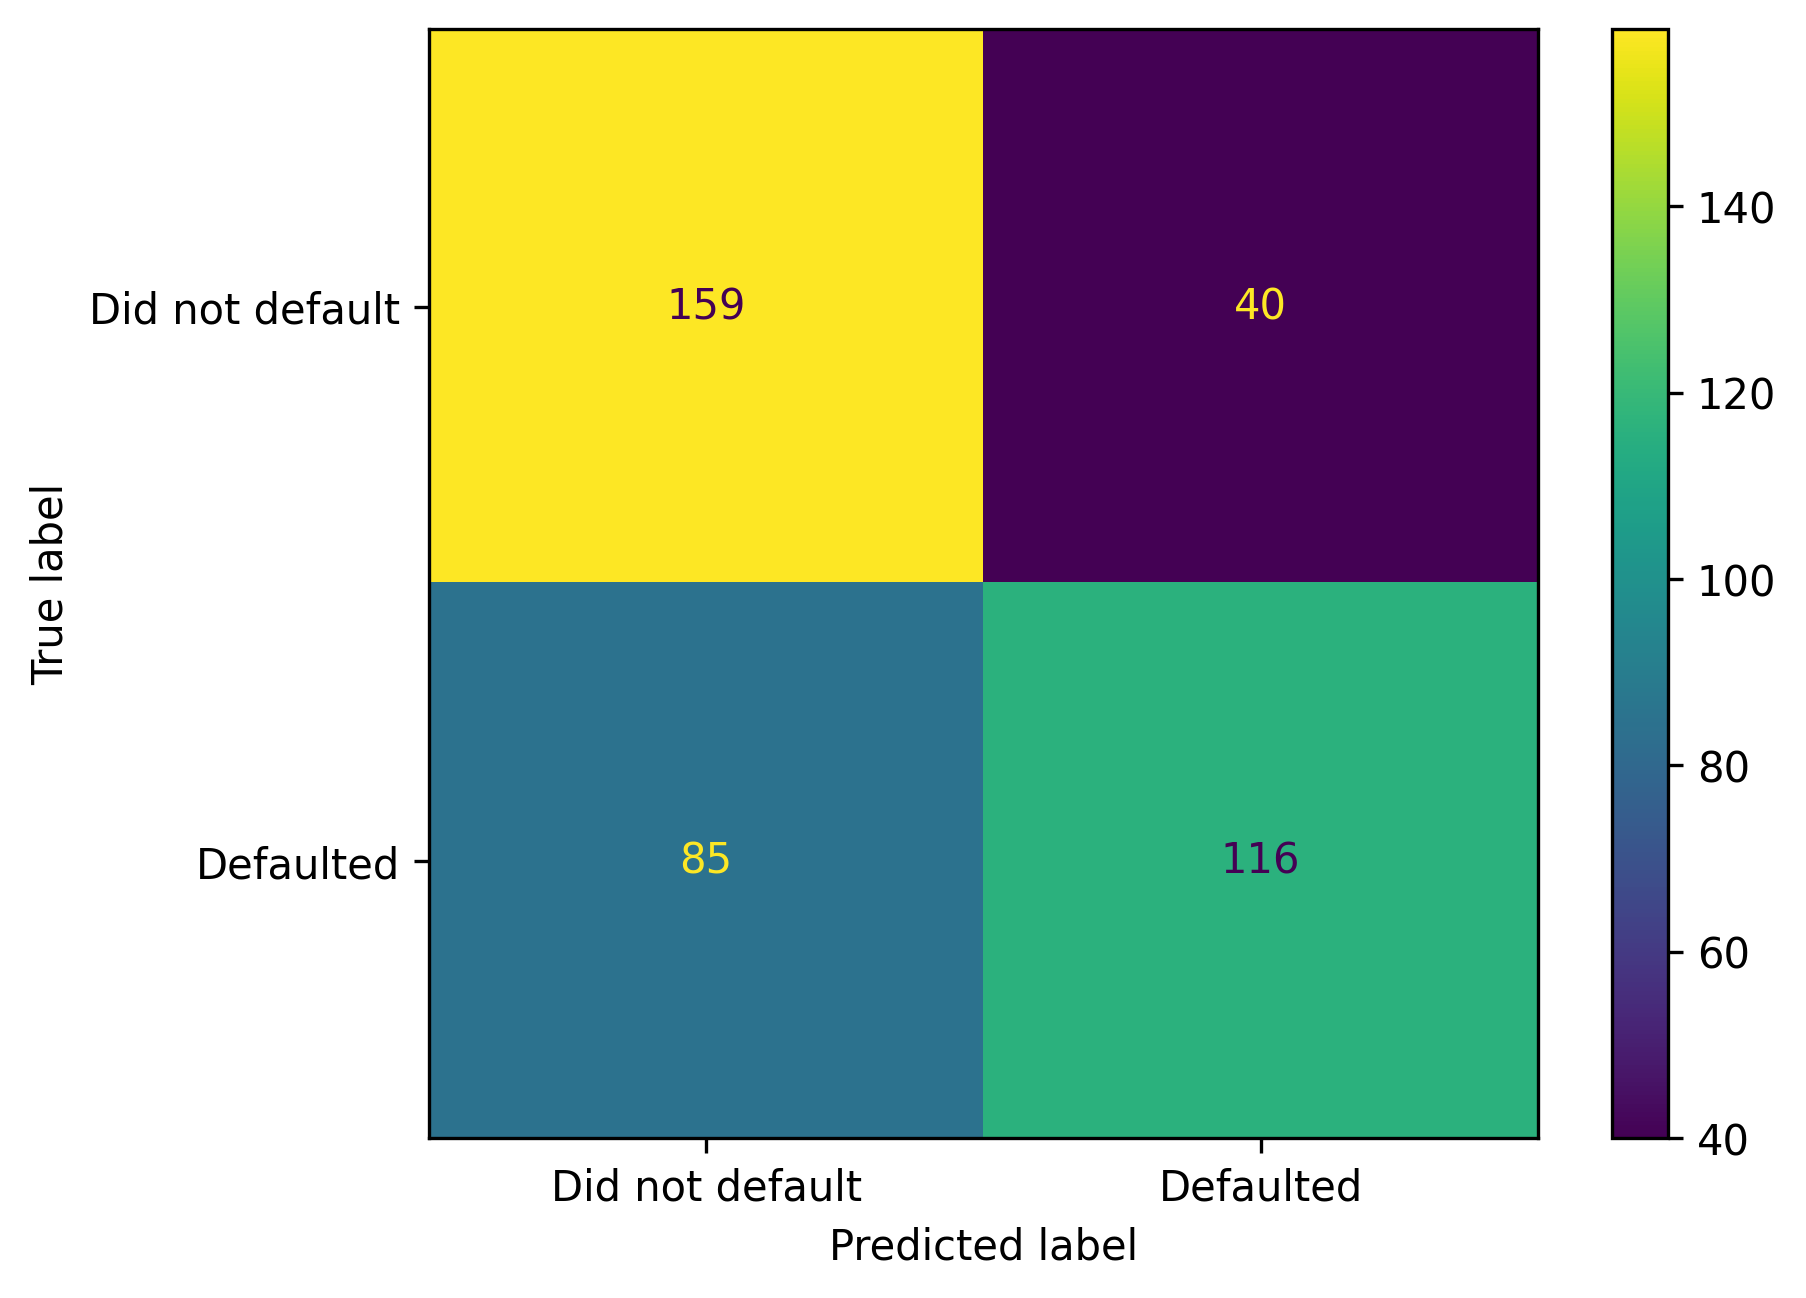
\includegraphics[width=0.7\textwidth]{../figures/confusion_matrix_post_gridSearch.png}
    \caption{Confusion Matrix After Grid Search.}
    \label{fig:confusion-post-grid}
\end{figure}

\begin{table}[H]
\centering
\caption{Kernel Comparison Results}
\label{kernel-results}
\begin{tabular}{@{}lcccccc@{}}
\toprule
\textbf{Kernel} & \textbf{Accuracy} & \textbf{Precision} & \textbf{Recall} & \textbf{F1-Score} & \textbf{Runtime (s)} & \textbf{Best Hyperparameters (C, $\gamma$)} \\ \midrule
Linear          & 0.6525            & 0.7095             & 0.5224          & 0.6017            & 0.2457              & (1, Scale)                                    \\ 
Polynomial      & 0.6700            & 0.7226             & 0.5572          & 0.6292            & 0.0629              & (10, 0.01)                                   \\ 
RBF             & 0.6875            & 0.7436             & 0.5771          & 0.6499            & 0.0634              & (1, 0.01)                                    \\ 
Sigmoid         & 0.6450            & 0.7007             & 0.5124          & 0.5920            & 0.0891              & (100, 0.001)                                 \\ \bottomrule
\end{tabular}
\end{table}

\begin{figure}[H]
    \centering
    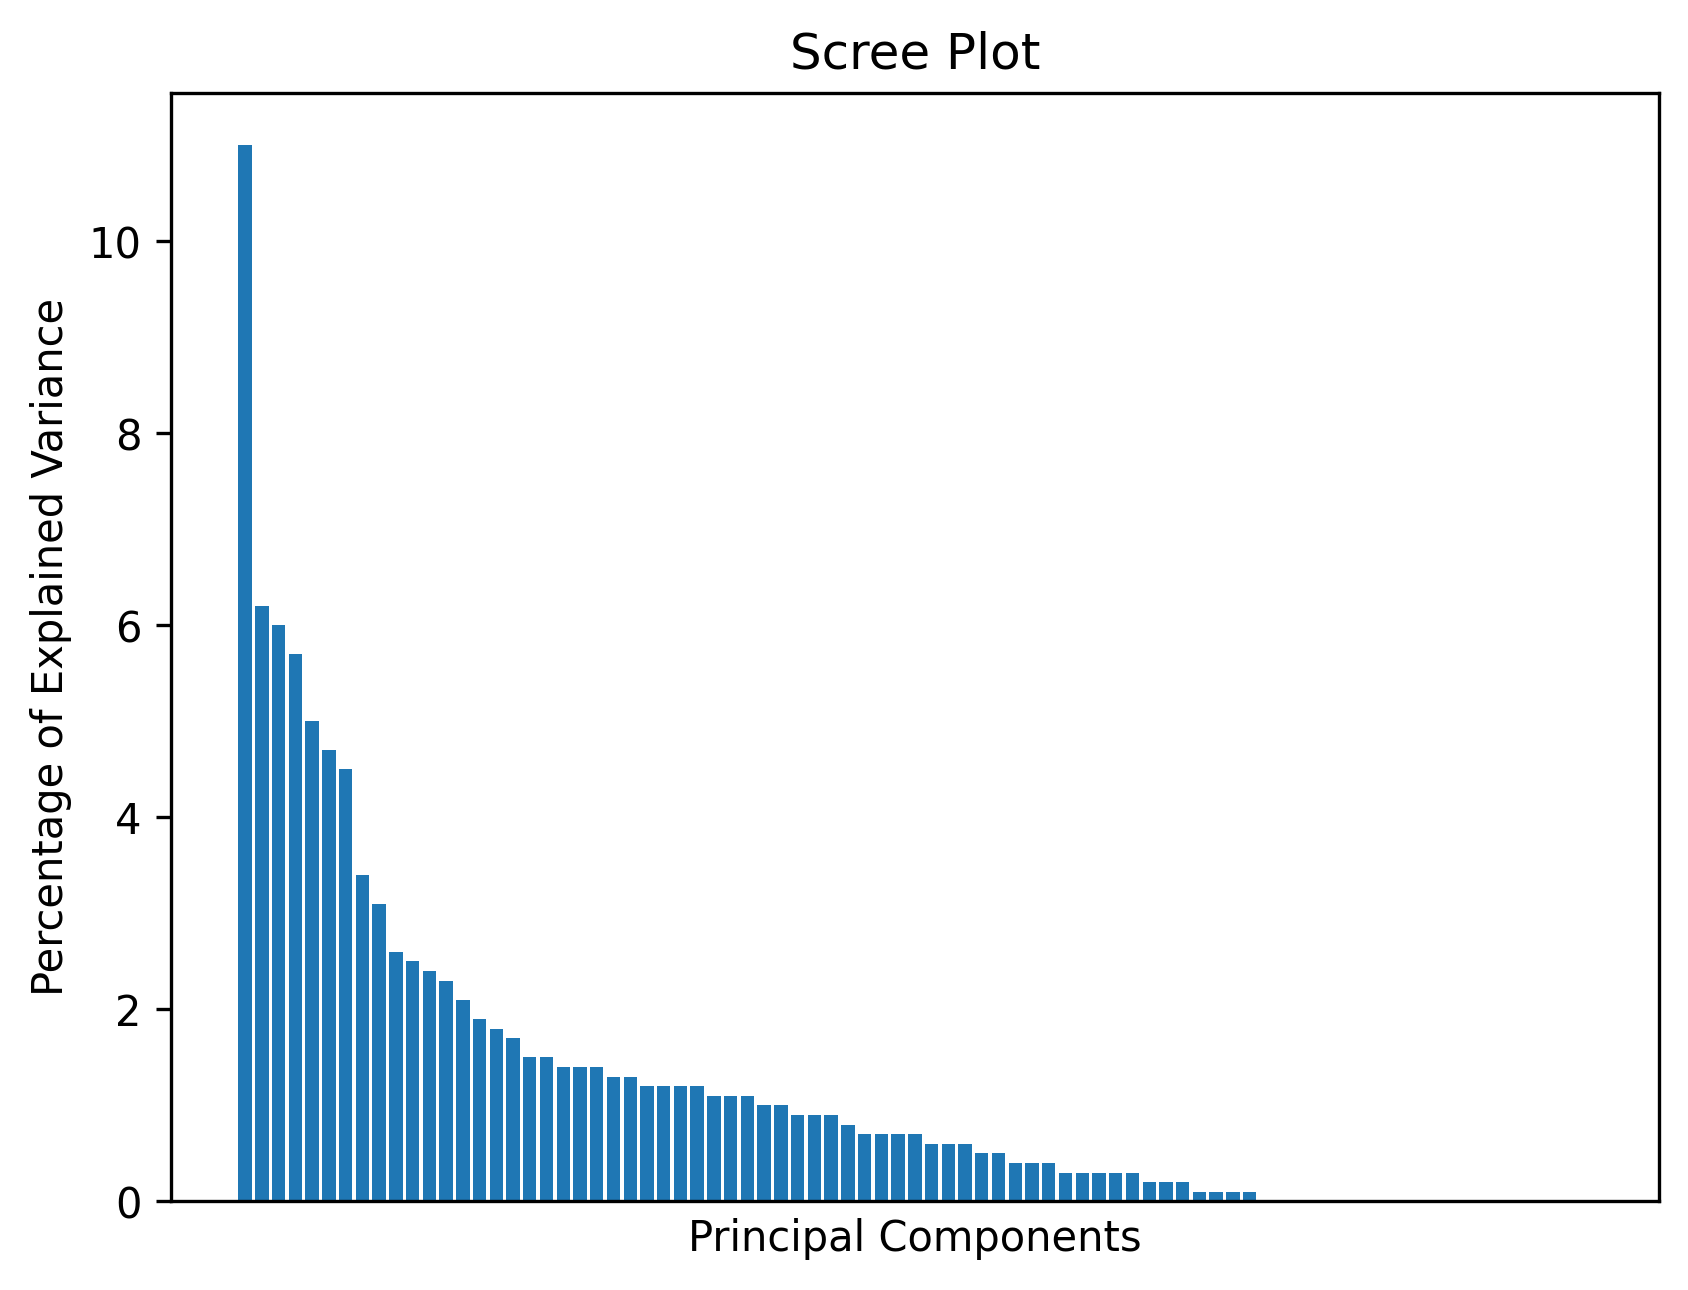
\includegraphics[width=0.7\textwidth]{../figures/scree_plot.png}
    \caption{Scree Plot Showing Percentage of Explained Variance.}
    \label{fig:scree-plot}
\end{figure}

\begin{figure}[H]
    \centering
    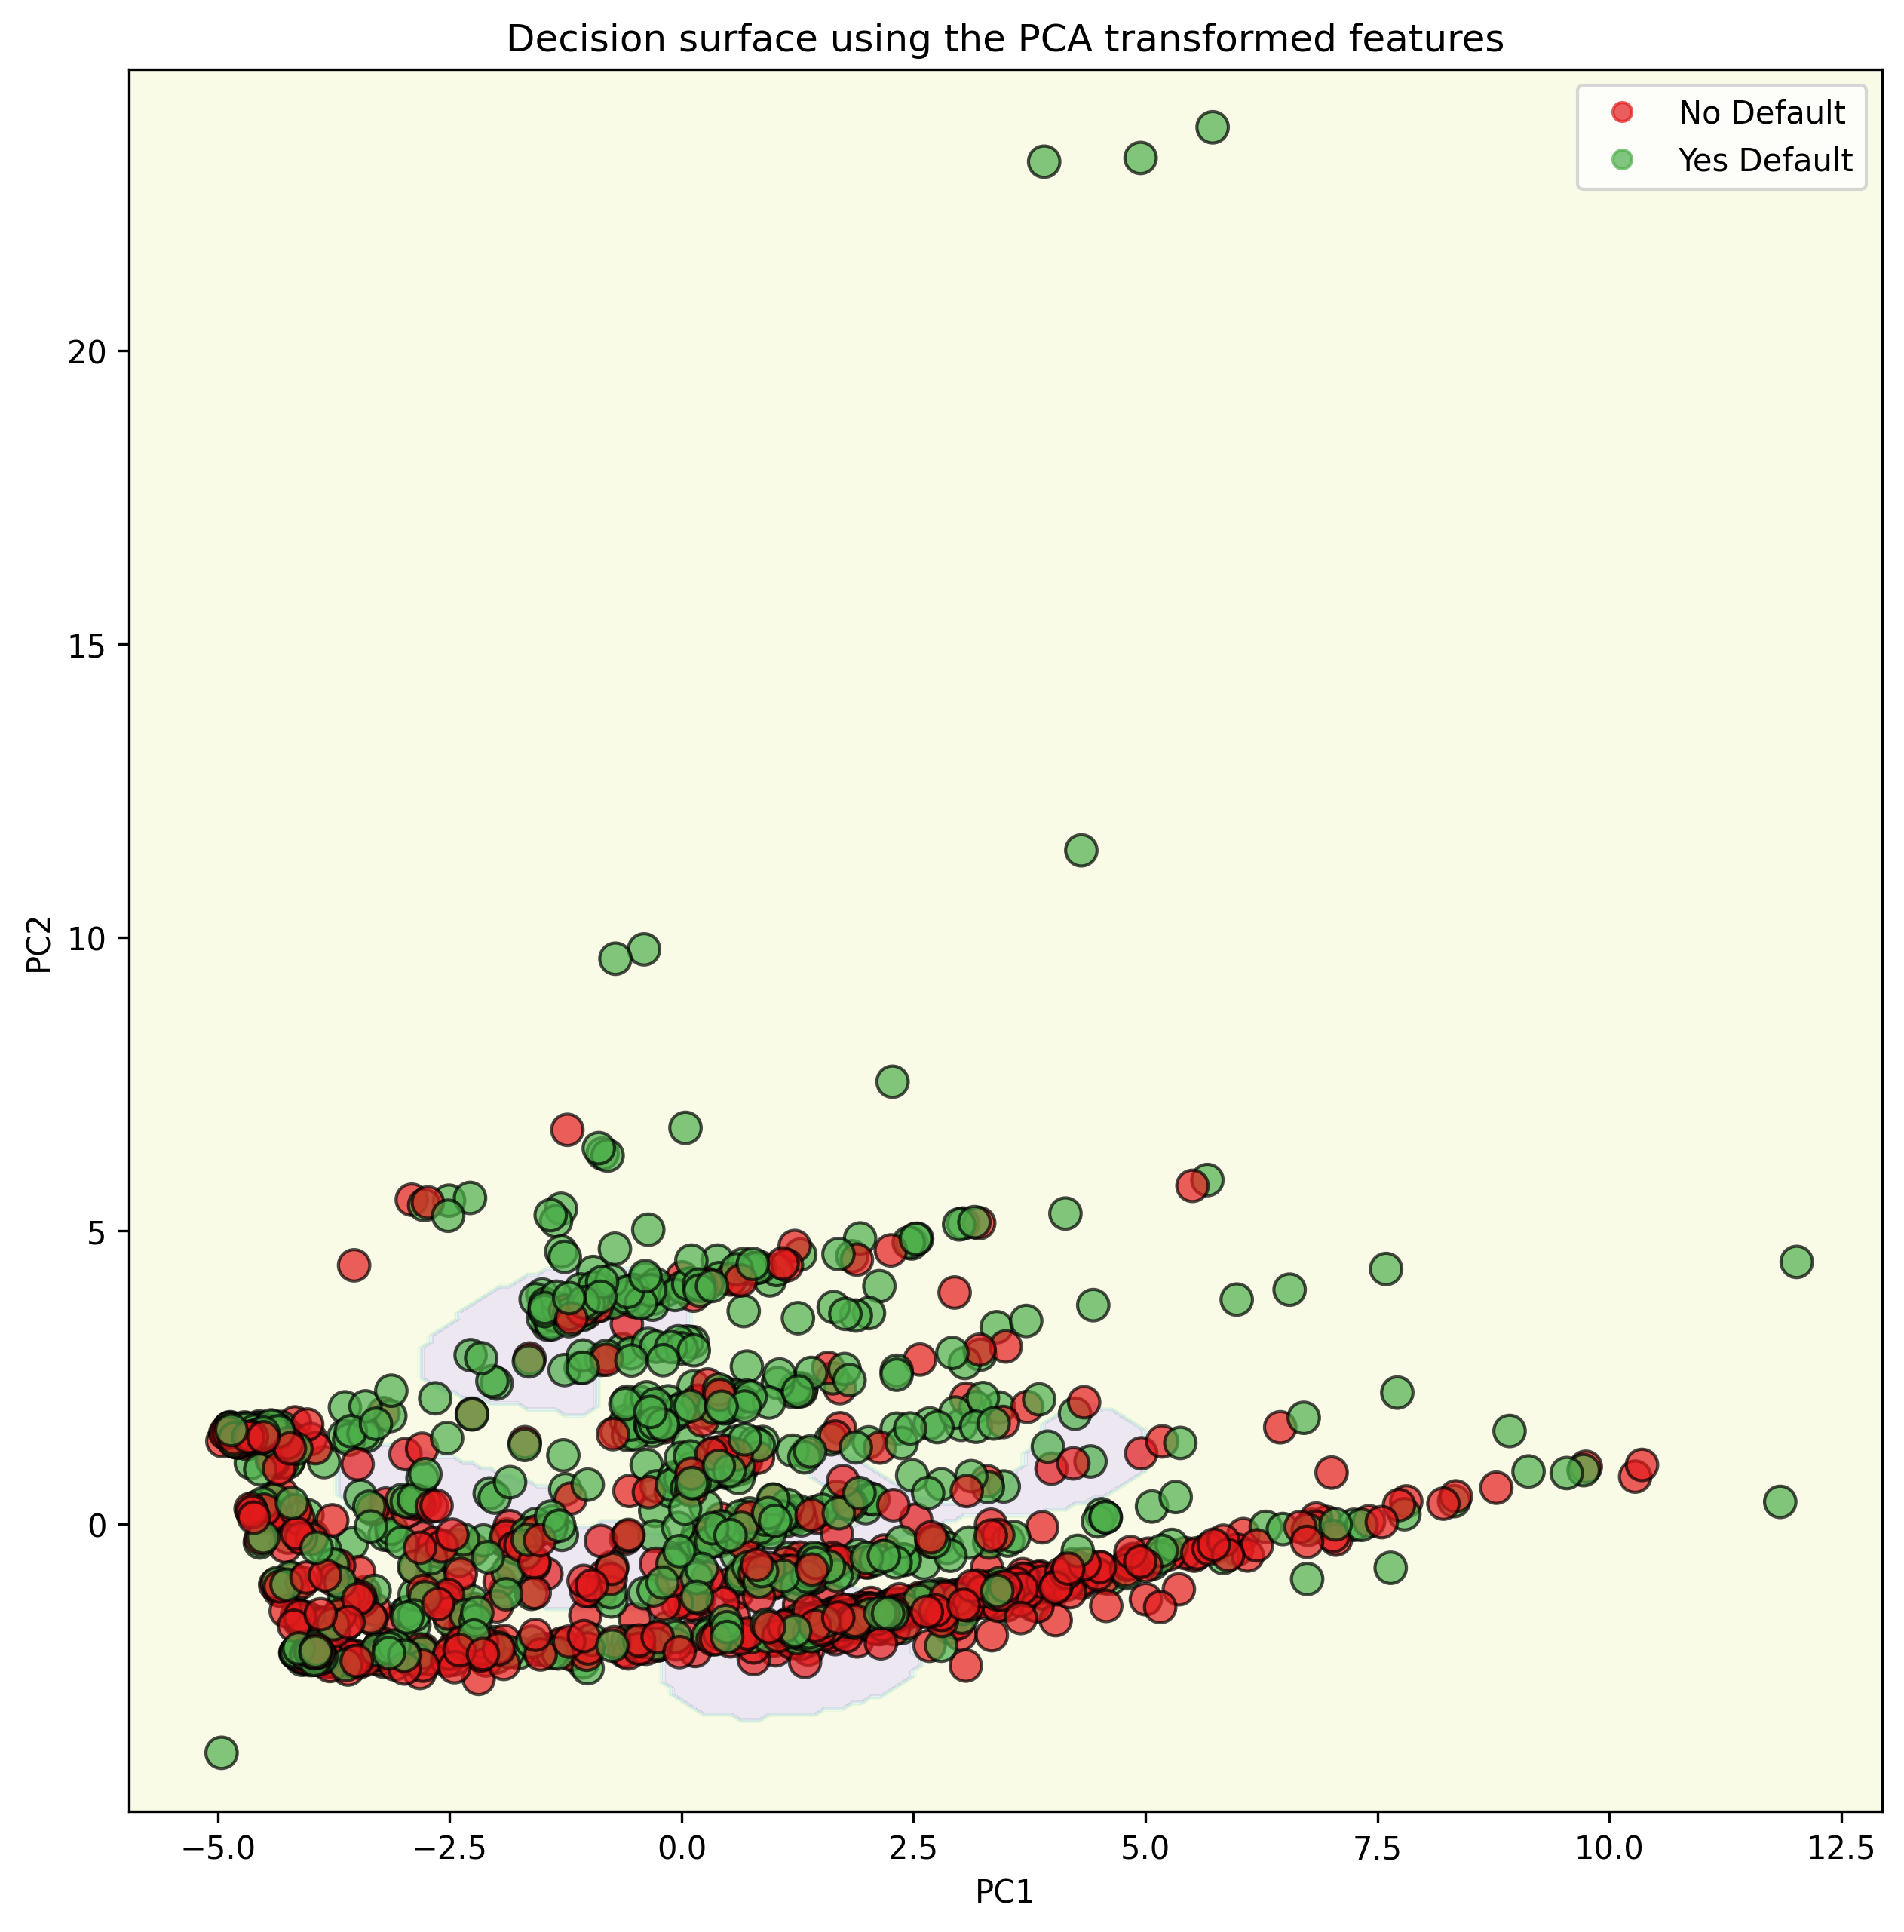
\includegraphics[width=0.7\textwidth]{../figures/decision_surface_pca.png}
    \caption{Decision Surface Using PCA Transformed Features.}
    \label{fig:decision-surface}
\end{figure}

\section{Discussion}
The results highlight the importance of kernel selection in Support Vector Machines (SVMs) for binary classification tasks. Among the evaluated kernels, the radial basis function (RBF) kernel emerged as the 
best performing option, achieving an accuracy of 68.75\%. This performance underscores the RBF kernel's strength in mapping data into higher-dimensional spaces, enabling it to capture nonlinear decision boundaries. 
However, the achieved accuracy is relatively modest, raising questions about the suitability of SVMs for this particular dataset. While the polynomial kernel showed competitive performance with an accuracy of 67.00\%, 
its sensitivity to parameter tuning limited its robustness. The linear kernel underperformed, achieving an accuracy of only 65.25\%, which can be attributed to its inability to handle the nonlinear structure of the data. 
The sigmoid kernel, with its complex parameterization, struggled to converge effectively and yielded the lowest accuracy of 64.50\%.

The relatively low accuracy across all kernels suggests that SVMs, while powerful, may not be the optimal model for this task. The imbalanced and high-dimensional nature of the dataset likely contributed to the suboptimal performance. 
Although hyperparameter tuning via grid search improved the models, as evidenced by the enhanced confusion matrix after optimization (Figure~\ref{fig:confusion-post-grid}), the gains were incremental and insufficient to achieve high accuracy. 
This indicates that the inherent characteristics of the dataset—such as overlapping class distributions and complex relationships among features—pose challenges that SVMs alone may not effectively address.

The PCA visualization of the decision boundary (Figure~\ref{fig:decision-surface}) provided insights into the separability of the classes, but the limited explained variance from the first two principal components (Figure~\ref{fig:scree-plot}) 
suggests that the majority of the dataset's complexity lies in higher dimensions. This highlights a limitation of using PCA for interpretability and suggests that other dimensionality reduction techniques, could provide more nuanced insights into the data's structure.

\section{Conclusion}
This study demonstrates the effectiveness of support vector machines for credit card default prediction. The findings emphasize the importance of kernel selection, with the RBF kernel offering the best performance among the four kernels evaluated. 
Hyperparameter tuning further enhanced classification accuracy, though its impact was secondary to the choice of kernel. Future work could explore additional dimensionality reduction techniques, alternative kernel functions, and the application of SVMs to larger, more diverse datasets.
In summary, while SVMs demonstrated some utility in this study, the results indicate that they may not be the most effective model for predicting credit card default. The modest accuracy, despite careful preprocessing and hyperparameter tuning, 
underscores the need for exploring alternative machine learning models and techniques to better address the complexity of the dataset and improve predictive performance.

\section*{References}
\begin{itemize}
    \item Chang, C. and Lin, C. (2011). LIBSVM: A library for support vector machines. \textit{ACM Transactions on Intelligent Systems and Technology}, 2(3), 27.
    \item UCI Machine Learning Repository: Default of Credit Card Clients Dataset. Available at \url{https://archive.ics.uci.edu/ml/datasets/default+of+credit+card+clients}.
    \item Cortes, C., and Vapnik, V. (1995). Support-Vector Networks. \textit{Machine Learning}, 20(3), 273–297.
\end{itemize}

\end{document}
